\begin{itemize}

\item Một miền cần chia đủ nhỏ để phù hợp với một nhóm cụ thể. Để đạt được điều này, chúng ta cần xác định rõ ranh giới giữa các ngữ cảnh.

\item Bối cảnh giới hạn (Bounded Context) giúp định rõ các ranh giới, chia miền thành các phần độc lập để giải quyết sự phức tạp trong mô hình doanh nghiệp.

\item Bối cảnh giới hạn thể hiện phạm vi kinh doanh của dịch vụ.

\item Bối cảnh giới hạn tạo ra các mô hình khác nhau cho các lĩnh vực khác nhau của miền.

\item Bối cảnh giới hạn tương ứng với một nhóm cụ thể trong tổ chức.

\end{itemize}

Ví dụ: Đây là 1 bối cảnh giới hạn của 1 ngân hàng xxxxxxx.

\begin{figure}[H]

\centering

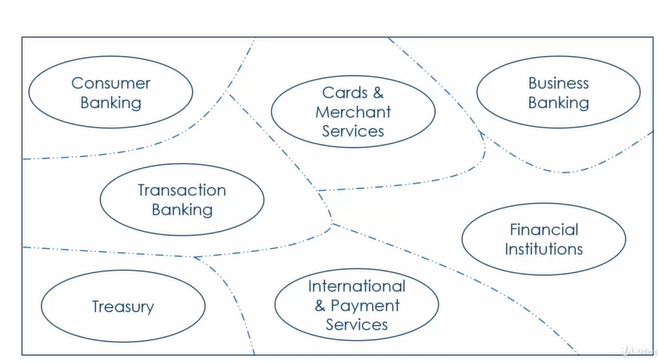
\includegraphics[width = 0.8\textwidth]{pictures/BoiCanhGioiHan/main.png}

\caption{vvn20206205}

\end{figure}

\subsubsection{Một vài hướng xác định bối cảnh giới hạn:}

\begin{itemize}

\item Việc xác định bối cảnh giới hạn được điều chỉnh bởi sự gắn kết giữa các miền phụ.

\item Dựa vào sơ đồ cấu trúc tổ chức của doanh nghiệp.

\item Dựa vào modules của các ứng dụng kiến trúc nguyên khối (nếu việc phân chia tốt).

\item Dựa vào trách nhiệm và hoạt động của chuyên gia ngành.

\end{itemize}

\end{document}

%!<! - - Hướng dẫn 5/10 - - >

% %!<! - - Bounded Context: https:// thiết kế hướng miền - practitioners.com/home/glossary/bounded - context - - >

% %!<! - - Bounded Context Relationships : https:// thiết kế hướng miền - practitioners.com/bounded - context - relationship - - >

Mối quan hệ bối cảnh giới hạn

Trong Thiết kế hướng miền (thiết kế hướng miền), bối cảnh giới hạn là ranh giới trong đó một mô hình miền cụ thể tồn tại và hợp lệ. Các ngữ cảnh giới hạn giúp xác định phạm vi của mô hình miền và thiết lập sự hiểu biết rõ ràng về ngôn ngữ được sử dụng trong ngữ cảnh đó.

Các bối cảnh giới hạn phải độc lập trong bối cảnh riêng của chúng, nhưng chúng vẫn có thể cần tương tác với các bối cảnh giới hạn khác để hoàn thành trách nhiệm của chính chúng. Mặc dù chúng độc lập về mặt mô hình nhưng chúng có thể cần giao tiếp với các bối cảnh giới hạn khác để trao đổi thông tin hoặc cộng tác trong một số nhiệm vụ nhất định. Vì vậy các bối cảnh giới hạn có thể có mối quan hệ với nhau. Những mối quan hệ này rất quan trọng vì chúng giúp xác định sự tương tác giữa các phần khác nhau của hệ thống, cũng như thiết lập ranh giới và trách nhiệm giữa các nhóm khác nhau làm việc trên cùng một hệ thống. Có một số loại mối quan hệ bối cảnh giới hạn, bao gồm:

Quan hệ đối tác : Đây là mối quan hệ trong đó hai hoặc nhiều bối cảnh giới hạn cộng tác và chia sẻ thông tin. Mối quan hệ hợp tác có thể đạt được thông qua một sự kiện tích hợp hoặc bằng cách gọi một dịch vụ.

Hạt nhân được chia sẻ : Trong mối quan hệ này, hai bối cảnh giới hạn chia sẻ một lược đồ mô hình, mã hoặc CSDL chung. Các thành phần được chia sẻ phải ổn định, hoàn thiện và được cả hai nhóm đồng ý. Những thay đổi được thực hiện đối với các thành phần dùng chung cần phải được phối hợp cẩn thận để đảm bảo chúng không phá vỡ chức năng của bối cảnh khác.

Khách hàng - Nhà cung cấp : Đây là mối quan hệ trong đó một bối cảnh giới hạn cung cấp dịch vụ hoặc dữ liệu cho bối cảnh khác. Bối cảnh khách hàng dựa vào bối cảnh nhà cung cấp để có những khả năng hoặc dữ liệu nhất định. Những thay đổi trong bối cảnh nhà cung cấp có thể tác động đến bối cảnh khách hàng, vì vậy điều quan trọng là phải quản lý mối quan hệ này một cách cẩn thận.

Người theo chủ nghĩa tuân thủ : Mối quan hệ này tồn tại khi một bối cảnh giới hạn tuân theo cùng một ngôn ngữ và khái niệm phổ biến như một bối cảnh giới hạn khác. Điều này đảm bảo rằng giao tiếp giữa hai bối cảnh là rõ ràng và rõ ràng.

Lớp chống đổ vỡ : Đây là mối quan hệ trong đó ngữ cảnh được giới hạn sử dụng một lớp để dịch giữa ngôn ngữ của chính nó và ngôn ngữ của ngữ cảnh giới hạn khác. Điều này cho phép hai ngữ cảnh giao tiếp với nhau ngay cả khi chúng có từ vựng hoặc mô hình khác nhau.

Dịch vụ máy chủ mở : Mối quan hệ này xảy ra khi một bối cảnh giới hạn hiển thị một API công khai, mở mà các ngữ cảnh khác có thể sử dụng. Điều này cho phép các ngữ cảnh khác tận dụng chức năng của ngữ cảnh máy chủ theo cách được tiêu chuẩn hóa.

Ngôn ngữ được xuất bản : Trong mối quan hệ này, một ngữ cảnh giới hạn sẽ xuất bản từ vựng và mô hình của nó cho các ngữ cảnh khác sử dụng. Điều này hữu ích khi nhiều bối cảnh cần cộng tác nhưng không muốn tích hợp trực tiếp. Ngôn ngữ được xuất bản đảm bảo rằng ý nghĩa của các thuật ngữ nhất quán trong mọi ngữ cảnh.

Các cách riêng biệt : Mối quan hệ này đề cập đến tình huống trong đó hai hoặc nhiều bối cảnh giới hạn không còn có mối quan hệ với nhau và các nhóm chịu trách nhiệm về chúng chọn làm việc độc lập.

% %!<! - - Bounded Context Relationships : https:// thiết kế hướng miền - practitioners.com/bounded - context - relationship - - >

% %!<! - - Bounded Context Relationships : https:// thiết kế hướng miền - practitioners.com/bounded - context - relationship - - >